% Conditional compilation
\providecommand{\setflag}{\newif \ifwhole \wholefalse}
\setflag

\documentclass[12pt,a4paper]{article}

\usepackage{booktabs} % Nice tables
\usepackage{graphicx}
\usepackage[top=1.1in, bottom=1.25in, left=1.25in, right=1.25in]{geometry}
\usepackage{hyperref}
\usepackage{xcolor}

% Remove ugly boxes around hyperlinks
\hypersetup{%
    colorlinks,
    linkcolor={red!80!black},
    citecolor={green!50!black},
    urlcolor={blue!80!black}
}

\parindent 0pt
\parskip 6pt

\begin{document}
\begin{center}
\Large
Computer Science Tripos -- Part II -- Project Proposal\\[4mm]
\LARGE
Exploring the structure of mathematical theories using graph databases\\[4mm]

\large
Dhruv C.~Makwana, Trinity College

Originator: Dr.~Timothy G.~Griffin

% \today
\end{center}

\vspace{5mm}

\textbf{Project Supervisor:} Dr.~Timothy G.~Griffin

\textbf{Directors of Studies:} Dr.~Frank Stajano \& Dr.~Sean B.~Holden

\textbf{Project Overseers:} Dr.~David J.~Greaves  \& Prof.~John Daugman

% Main document
\section*{Introduction and Description of the Work}
This project aims to (a) represent Coq libraries as Neo4j (graph) databases
and (b) create a library of Neo4j queries with the goal of highlighting
the structure and relationship between the representations of the proof-objects.

Mathematics textbooks aimed at professionals/researchers follow a well-established
rhythm: define some constructions and some properties on them and prove
theorems on both, with lemmas, corollaries and notation interspersed
throughout. Such a presentation is concise but limiting: it is linear; it forces
the reader to keep track of dependencies such as implicit assumptions, previously
defined results and the types and conventions behind any notation used;
and it offers little opportunity to consider and compare different approaches
for arriving at a result (i.e.\ number of assumptions, number of steps, some
notion of the importance of a result such as number of uses by later
results).

With the increasing popularity of interactive theorem-provers such as Coq
\cite{Coq:manual} and Isabelle \cite{nipkow2002isabelle}, many mathematical theories
(such as the formidably large Feit-Thompson Odd Order Theorem
\cite{peterfalvi2000oot, bender1994oot}) have been \cite{gonthier2013oot} or are being
translated and formalised into machine-checked proof-scripts. However, these
proof-scripts on their own inherit the same disadvantages as the aforementioned
textbooks, as well as some new ones: they are usually more verbose and explicit
and are primarily designed for automation/computation than readability. The
former (usually out of necessity to convey to the computer the intended
meaning) leads to unnecessary ``noise'' in the proof and the latter departs
from the vocabulary or flow a natural-language presentation may have.

The database world is currently experiencing a tremendous explosion of creativity
with the emergence of new data models and new ways of representing and querying
large data sets. \emph{Graph databases} have been developed to deal with highly
connected data sets and path-oriented queries. That is, graph databases are
optimised for computing transitive-closure and related queries, which pose a
huge challenge for traditional, relational databases.

A graph-based approach to the representation and exploration of the structure of
proof-objects would	be a far more natural expression of the complex
relationships (i.e.\ chains of dependencies) involved in
constructing mathematical theories. Questions such as ``What depends on this
lemma and how many such things are there?'' or ``What are the components of
this definition?'' could thus be expressed concisely (questions which are not
even expressible with standard relational databases systems such as
SQL). A popular graph database, Neo4j~\cite{neo4j} with an expressive query
language \emph{Cypher} will be used for this project.
	
\section*{Resources Required}

\subsection*{Software}
Several components of software will be required for executing this project, all
of which are available for free online.

For using the proof-scripts, the Coq proof assistant will be required, as well
as the Proof General proof assistant
(\href{http://proofgeneral.github.io/}{\texttt{proofgeneral.github.io/}}) for the Emacs
(\href{http://www.gnu.org/software/emacs/}{\texttt{www.gnu.org/software/emacs/}})
text-editor.

For writing the plug-in to access Coq proof-objects, the parser and associated
modules in the source code will be required
(\href{http://github.com/coq/coq}{\texttt{github.com/coq/coq}}) written in the OCaml
programming language (\href{http://ocaml.org}{\texttt{ocaml.org}}) with the OCaml's
Package Manager OPAM (\href{http://opam.ocaml.org}{\texttt{opam.ocaml.org}}).

For building the library of (Cypher) queries, Neo4j Community Edition will be
used.

\subsection*{Hardware}
Implementation and testing will be done on both Windows 10 and a Linux Virtual
Machine as appropriate and convenient on a Surface Pro 3 (Intel Haswell i7-4650U
1.7-3GHz, 8GB RAM, 512GB SSD) with a personal GitHub account and physical backup
drive (Seagate 1TB) making hourly backups using Windows' File History.

\section*{Starting Point}
Some existing tools offer part of the solutions: these will be used and
combined as appropriate. A large part of the project will rely on my knowledge of
OCaml and Coq usage and internals.

Coq-dpdgraph
(\href{http://github.com/Karmaki/coq-dpdgraph}{\texttt{github.com/Karmaki/coq-dpdgraph}})
is a tool which analyses dependencies between \emph{compiled} Coq proofs. As
such, desirable information about notation, tactics, definitions and the
relationship between a type and its constructors is lost.

Coqdep is a utility included with Coq which analyses dependencies \emph{at the
module level} by tracking {\tt Require} and {\tt Import} statements.

Coq SerAPI
(\href{http://github.com/ejgallego/coq-serapis}{\texttt{github.com/ejgallego/coq-serapis}})
is a work-in-progress library and communication protocol for Coq designed to
make low-level interaction with Coq easier, especially for IDEs. It has a
starting point for gathering some statistics of proof-objects in a project.

All of these tools have the same disadvantage: they present information statically,
with no way to query and interact with the information available.

\section*{Substance and Structure of the Project}
\begin{figure}[tb]
	\centering
	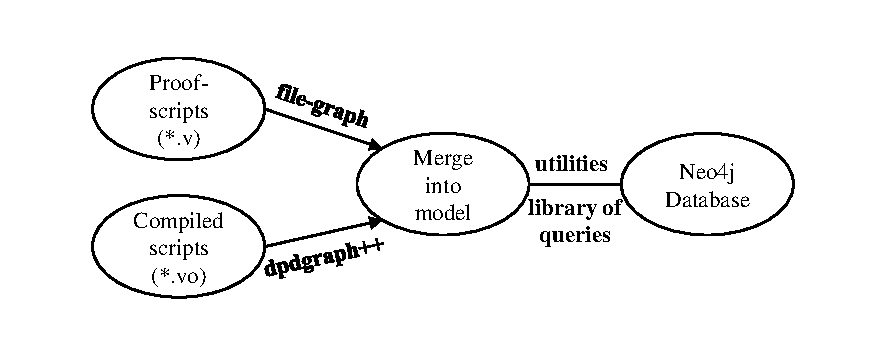
\includegraphics[width=\textwidth, page=1]{proposal/proposal-project-structure-diagram.pdf} 
  \caption{System Components}\label{fig:propstructure}
\end{figure}

The project will have three major parts, as shown in Figure~\ref{fig:propstructure}.

\subsection*{Processing Compiled Files}
First, using coq-dpdgraph as a starting point, a tool which expresses a
compiled proof-script as CSV files (shown as ``dpdgraph++'' in the diagram).
Finding what information can and should be extracted will be an iterative
process. Although coq-dpdgraph is functional, it is very basic with no way of
even relating the relationship between a (co-)inductive type and its
constructors, hence much work is to be done to even come close to utilising the
full potential of compiled proof-scripts.

\subsection*{Processing Source Code Directly}
Second, using Coq's sophisticated extensible-parser, to parse, gather and
convert to CSV files the desirable but missing information
coq-dpdgraph does not extract (shown as ``file-graph'' in the diagram). An
interesting feature of Coq's parser is that it allows new constructs and
notation to be defined: this is used heavily in some projects and therefore
poses a great challenge for simply understanding and using the parser
effectively.

\subsection*{Extraction and Analysis Tools}
Lastly, writing utilities to automate analysis of Coq files and importing them into
Neo4j and libraries of queries to run on imported data in Neo4j. Since it is not
known what sort of data can be extracted and what will be useful or interesting to
know, modelling the data -- in this case the structure and objects of a mathematical
proof -- will be an non-trivial task which will be tackled iteratively.

\subsection*{Extensions}

Extensions for this project will come from the process of adapting the project to
be compatible with SSReflect~\cite{gonthier2015ssr}, part of the Mathematical
Components set of tools for Coq. These set of tools use low-level hooks in the
Coq plugin system to significantly alter the specification and computation of
proofs. As such, although they allow for large-scale projects to be formalised
more easily, they are non-standard and would thus be very difficult to support
fully.

\ifwhole\newpage\else\fi%
\section*{Success Criteria}

Alongside a planned and written dissertation describing the work done, the
following criteria will be used to evaluate the success of this project:

\begin{enumerate}

	\item A schema of attributes and relations for each proof-object is defined.
	\item Programs which convert proof-scripts and compiled proofs to CSV files
		  are implemented.
	\item A library of queries in order to manipulate and explore the proof-objects
		  is implemented.
	\item These new sets of tools are shown to have more capabilities and perform
		  comparably to existing tools for exploring mathematical theories.

\end{enumerate}

\newpage
\section*{Timetable and milestones}
\vspace*{\fill}

\begin{table}[h]
\centering
\begin{tabular}{ll}
    \toprule

    Date & Milestone \\

    \midrule

	% October
	21-10-2016	&	Complete Project Proposal \\ \\
          
	% November
	04-11-2016	&	Finish a prototype compiled-to-CSV tool. \\ 
				&	Get familiar with Neo4j Cypher. \\
				&	Understand how to use the Coq parser. \\ \\

	18-11-2016	&	Refine compiled-to-CSV tool: tests and documentation. \\
				&	Explore queries possible and start the library. \\
				&	Begin work on translating Coq constructs from proof-scripts. \\ \\

	% December
    02-12-2016	&	Finish a prototype script-to-CSV tool. \\ \\

    16-12-2016	&	Test and document script-to-CSV tool. \\ \\

    30-12-2016	&	Begin work on integrating tools into one workflow. \\ \\

	% January
	13-01-2017	&	Stabilise and document whole project so far. \\
				&	Prepare presentation for CoqPL Conference. \\ \\

    27-01-2017	&	Look at SSReflect and evaluate changes to be made. \\ \\

	% February
    10-02-2017	&	Incorporate changes from feedback/new features. \\ \\

    24-02-2017	&	Test and document the new features. \\ \\

	% March
	10-03-2017	&	Write Introduction, Preparation and Implementation chapters. \\ \\

    24-03-2017	&	Fix bugs/unexpected problems. \\ \\
    
	% April
    07-04-2017	&	Write Evaluation and Conclusion chapters. \\ \\

    21-04-2017	&	Fix bugs/unexpected problems. \\ \\
    
	% May
	05-05-2017	&	Complete Dissertation (references, bibliography, appendix, formatting). \\

  \bottomrule

\end{tabular}
\end{table}
\vspace*{\fill}

\ifwhole \else

  \newpage
  \phantomsection{} % Stop hyperlinks from going to the wrong page
  \bibliographystyle{plain}
  \bibliography{src/dissertation.bib}
  \cleardoublepage{}

\fi

\end{document}
